\paragraph{Relação força-frequência das unidades motoras}
Na Figura 2 observa-se que a relação força-frequência apresenta uma região linear para os três tipos de unidades motoras; porém, a força tetânica de cada unidade motora é diferente, sendo que as unidades motoras dos tipos S, FR e FF apresentaram forças tetânicas máximas de aproximadamente 10 N, 15 N e 19 N, respectivamente. Uma maneira de avaliar a propriedade contrátil da UM é medindo-se a relação entre a amplitude máxima do abalo muscular e a força tetânica máxima (relação twitch/tétano) \cite{Kernell2006}. Nos modelos das unidades motoras dos tipos S, FR e FF estes valores foram de 16,8\%, 18,6\% e 11,1\%, respectivamente.

\begin{figure}[h]
  \centering
  \fbox{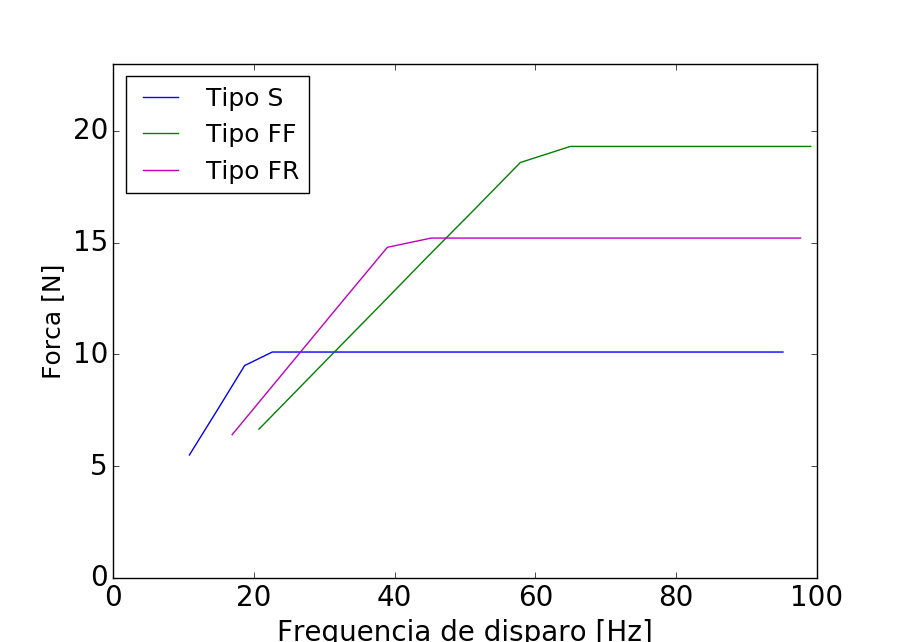
\includegraphics[width=7cm]{../figures/pdf/Forca-Freq.png}}
  \caption{Curva força-frequência para as unidades motoras dos tipos S, FR e FF}
  \label{fig:fig2}
\end{figure}

\paragraph{Princípio do tamanho e geração da força muscular}
Na parte inferior da Figura 3 estão indicados os instantes de disparos dos MNs de cada tipo (S em azul, FR em verde e FF em magenta). Os pontos na parte superior da Figura 3 indicam as frequências instantâneas de disparo dos MNs (mesmo código de cores) e a linha preta contínua representa a força total exercida pelo modelo simplificado de músculo. Nota-se que a unidade motora do tipo S é a primeira a ser recrutada, pois seu MN possui uma menor área celular (vide Tabela 1) e, consequentemente, uma maior resistência de entrada. Por outro lado, a unidade motora do tipo FF é a última a ser recrutada, pois o MN possui uma maior área celular e menor resistência de entrada. Além disso, observa-se nos resultados a ordem inversa de derrecrutamento, com a unidade motora de maior limiar (tipo FF) sendo derrecrutada primeiro e a de menor limiar (tipo S) por último.

\begin{figure}[h]
  \centering
  \fbox{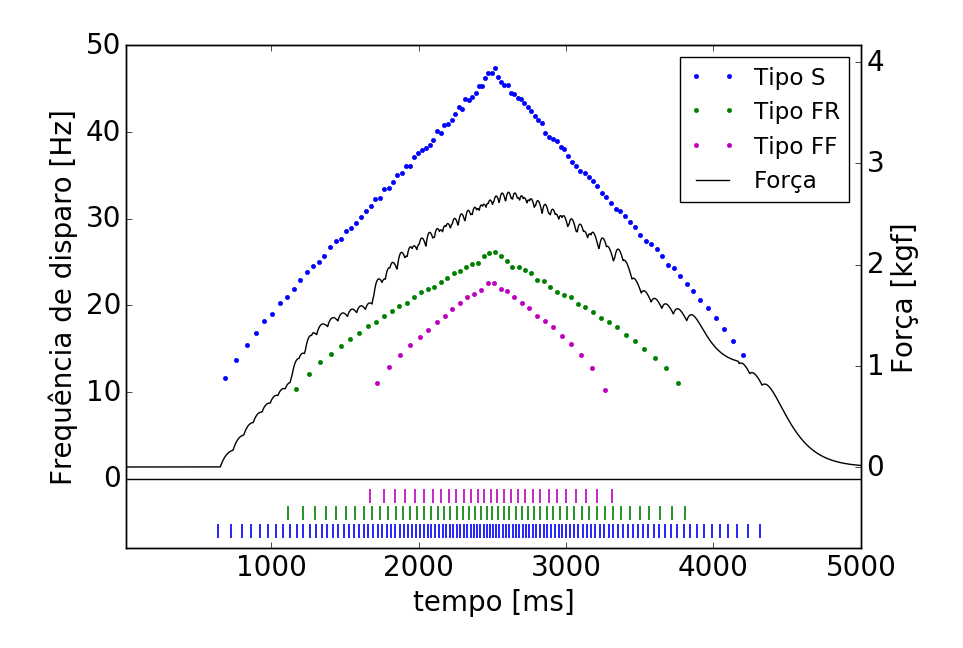
\includegraphics[width=7cm]{../figures/pdf/OnionSkin}}
  \caption{Mecanismos de controle e geração da força muscular. Os pontos coloridos representam as frequências de disparos dos MNs dos tipos S, FR e FF;os traços coloridos abaixo indicam os instantes de disparos dos PAs dos MNs; e a curva preta mostra avariação da força ao longo do tempo.}
  \label{fig:fig3}
\end{figure}

Do ponto de vista das frequências de disparos de PAs, observa-se que as unidades motoras recrutadas com um menor limiar atingem taxas de disparos maiores em comparação com as unidades motoras de maior limiar, para uma mesma magnitude da corrente de estimulação.

Quanto à geração da força muscular, nota-se na Figura 3 (linha preta) que a unidade motora do tipo S gera uma força relativamente pequena, mesmo com o aumento da sua frequência de disparos (pontos azuis) devido à menor amplitude dos abalos musculares e à força tetânica. À medida que novas unidades motoras são recrutadas (dos tipos FR e FF) a força aumenta, tanto pelo fato de estas unidades motoras produzirem abalos de maior magnitude, quanto por aumentarem as suas frequências de disparos (devido ao aumento da despolarização da membrana dos MNs pela corrente triangular). Observa-se, ainda, que quando as unidades motoras de maior limiar são recrutadas há um aumento na flutuação da força, pois os abalos não fundidos destas unidades motoras são mais evidentes.

%FIGURA